\documentclass[12pt,journal,compsoc]{IEEEtran}
% manually specify the path to it like:
% \documentclass[12pt,journal,compsoc]{../sty/IEEEtran}

% correct bad hyphenation here
\hyphenation{op-tical net-works semi-conduc-tor}
\usepackage{graphicx}
\usepackage{array}
\usepackage{tabularx}
\usepackage{color}
 \usepackage{comment}
 \usepackage{amssymb}
 \usepackage[ruled,vlined]{algorithm2e}
\providecommand{\SetAlgoLined}{\SetLine}
\SetKwIF{When}{WhenIf}{then}{when}{then}{else}{else}{end}

% Automatically equalizing two columns of last page
%\usepackage{flushend}

\usepackage[loose]{subfigure}
\usepackage{subfigure}
\usepackage{multirow}
\usepackage{multicol}

\usepackage{makeidx}  % allows for indexgeneration

%Aim: Mobicom

\begin{document}

\title{CLIMAX: Local medium access control adaptations for global efficiency}
% Climax : Cross-layer information for local MAC layer adaptations.

\author{Julien Beaudaux, Yuming Jiang% <-this % stops a space
\IEEEcompsocitemizethanks{\IEEEcompsocthanksitem J. Beaudaux and Y. Jiang are with the Department of Telematics, Norwegian University of Science and Technology (NTNU), Trondheim, Norway.\protect\\}% <-this % stops an unwanted space
%\thanks{Manuscript received April 19, 2005; revised December 27, 2012.}
}

% The paper headers
\markboth{}%
{Beaudaux \MakeLowercase{\textit{et al.}}: CLIMAX: Local medium access control adaptations for global wireless sensor networks efficiency}

\IEEEtitleabstractindextext{%
\begin{abstract}
Wireless sensor networks are now deployed for various purposes, ranging from eHealth to infrastructure monitoring. Each application implies specific performance requirement that have to be fulfilled for the deployment to be successful. Such requirements can take the form of, \textit{inter alia}, expected lifetime, minimal acceptable resiliency or maximal delay.
As the medium access control (MAC) configuration is typically the main factor impacting both communication performance and energy consumption, finding the most appropriate value for a considered application bears primordial importance.
% Yet, the quality of radio links is of variable and unpredictible nature, and two nodes assigned with different configurations may be deaf to each other. Thus, finding the best-suited configuration for each sensor node, complying with both performance requirements and deployment conditions is a very complex task. 
%At the moment, most solutions rely on an homogeneous MAC configuration, identical for all nodes and/or static over time. Yet, no homogeneous configuration can fullfill all application requirements throughout the deployment.
In the present paper, we introduce CLIMAX, a framework that locally determines the best-suited MAC configuration for each node in the network. CLIMAX continuously monitors the condition each node evolves in (e.g. traffic load, communication performance, energy consumption). This information is then coupled with a communication-behavior model, and translated into a multi-objective optimization problem, along with applicative requirements. The \textit{Pareto-solution} to this problem represents the best-suited node configuration to be adopted. 
We demonstrate to what extent CLIMAX helps adapting locally and automatically the MAC parameters to the current network status and reach applicative requirements.
%, its proper configuration bears primordial importance on the fulfillment of applicative requirements.
%Yet, the quality of radio links being of variable and unpredictible nature, finding the best-suited configuration for each sensor node, complying with both performance requirements and deployment conditions is a very complex task. 
%It thus bears primordial importance on the fulfillment of applicative requirements, and thereby the deployment's success or failure. 
%We first present a thorough empirical study of the interaction between MAC parameters, deployment conditions, and the fulfillment of applicative requirements. Based on these results, we demonstrate through intensive experimental campaigns to what extent CLIMAX helps reaching applicative requirements through local and dynamic sensor node’s MAC configuration adaptations. 
\end{abstract}

% Note that keywords are not normally used for peerreview papers.
\begin{IEEEkeywords}
Wireless sensor networks, Medium access control, Auto-adaptivity
\end{IEEEkeywords}}

\maketitle

\section{Introduction}
Ever since their debut over a decade ago, wireless sensor networks (WSN) have been conceived to be application-specific. Each deployment thus induces specific applicative requirements to be fulfilled. For instance, most patient monitoring systems \cite{dbg11wireless} require high quality of service (QoS) guarantees so that anomalies can be treated efficiently and in time. Other deployments, such as infrastructure monitoring \cite{kpc07health}, prioritize the network lifetime, in order to avoid the replacement of sensor nodes.

As communications typically stand for the main source of energy usage \cite{ass02wireless}, the Medium Access Control (MAC) layer has a direct impact on both those requirements. Indeed, typical WSN MAC protocols perform radio duty-cycling, periodically alternating between active and passive states at the radio scale to mitigate energy consumption, at the cost of communication performence. Its proper configuration is thus of prime importance.
For long, the sensor nodes MAC parameters (i.e. radio duty-cycle) were chosen \textit{a-priori}, based on deployment conditions (e.g. node placement, expected traffic model) \cite{dem10evolution, sensorscope10}. Thus, the same configuration was used throughout the network and/or the deployment period. This approach can provoke severe counter-performance in regards with applicative requirements, driving the network to ultimately fail \cite{sensorscope10, murphypotatoes06}. Indeed, the conditions the nodes evolve in may drastically vary both over time and position in the network \cite{linkstability12, addvalue13, tempimpact10}. Other solutions soved this issue by relying on the broadcasting throughout the network of a single configuration, decided centrally. However, this approach is hardly scalable and induce high communication overhead (i.e. network performance monitoring messages, broadcasting of the configuation).

%However, in typical WSN deployments, the communication performence may drastically vary both over time and from one node to another.

%, despite potential dynamics at work in the network (e.g. changes in traffic load, routing structure, link performance). 

% Yet, this approach can not cope with network dynamics and remains complex to implement, due to its close relation to the deployment itself.

% were configured \textit{a-priori}, based on deployment conditions (e.g. node placement, expected traffic model) \cite{dem10evolution, sensorscope10}. Yet, this approach can not cope with network dynamics and remains complex to implement, due to its close relation to the deployment itself.
%paper, we consider preamble sampling MAC protocols, that do so asynchronously.

%In numerous deployment, the lack of adaptability and drove the network to ultimately fail \cite{sensorscope10, murphypotatoes06}.


%Why MAC layer

%This approach is suited for static network, but can not cope with network dynamics, each node being configured once and for all, independently from condition changes.
%This caused several prior deployments experienced severe counter-performance due to such issue \cite{sensorscope10, murphypotatoes06}, each node being configured once and for all, independently from condition changes.

%One of the main reason to this is the high variability of WSN radio links over time. Low-power radio links such as those used for WSN communications are very sensitive, and even little environmental changes (e.g. temperature, humidity, human activity) can deeply affect the radio links quality (e.g. signal strengh, link symmetry) \cite{linkstability12, impactweather10}. Thus, statically configured networks may fulfill the applicative requirements at one time, but fail to adapt to network state change. 

%Yet, finding the best-suited MAC parameters for each node in real time depending on its current situation is a very complex task. 
In the present paper, we introduce the CLIMAX framework. CLIMAX relies on a different strategy, where the best-suited MAC parameters for each node is locally calculated and assigned in real time, depending on its current situation. Each sensor monitors its communication performance, energy usage and status in the network at runtime. This information is then coupled with an evolutive model depicting the local communication behavior, and provided along with applicative requirements as parameters to a multi-objective optimization problem (MOP). The \textit{Pareto-solution} to this problem represents the best-suited MAC configuration, that can be adopted immediately.

The present paper details the following contributions:

\begin{itemize}
	\item we demonstrate how high-level applicative requirements can be translated to a set of per-hop constrainsts that can be achieved locally, and how to efficiently and locally monitor the nodes communication-performance in real-time;
	\item we define a model that represents the expected behavior of communications in the network. This model is derived from experiments carried out prior to the \textit{in situ} deployment itself, and evolves in parallel with the performence experienced throughout the network deployment;
	\item we present the design and implementation of the CLIMAX framework, that makes use of the above-mentionned information and model to precisely calculate the best-suited MAC configuration according to the current situation;
	\item we detail our extensive evaluation campaign of the CLIMAX framework and the obtained results.
\end{itemize}

The remainder of the paper is organized as follows. In Section \ref{RW} we formulate the problem, motivate the need for a novel approach and present related work addressing this issue. Section \ref{contrib} describes each aspect of the CLIMAX framework and discusses how it helps obtaining locally the best-suited MAC configuration. Section \ref{results} presents
our evaluation and results, which are compared to the ones obtained by state-of-the-art solutions. Finally, Section \ref{ccl} draws the conclusions and suggests future work.

\section{Problem statement and related work}
\label{RW}

%Each WSN deployment is unique, and induce specific requirements. 

\subsection{Problem statement}
Each WSN deployment is unique and induce specific requirements. On one hand, some applications require a high level of quality of service, to ensure that the collected data is meaningful and can be exploited in time. On the other hand, energy consumption can also be a critical aspect, as sensor nodes usually have to operate autonomously for long periods, relying only on limited amount of energy (e.g. batteries, little-scale energy-harvesting devices).

As communications typically stand for the main source of energy usage \cite{ass02wireless}, their adequate management is of uttermost importance to both provide the network with the required QoS and lifetime guarantees. This problem is commonly addressed at the MAC layer, where specific protocols rely on radio duty-cycling to mitigate the radio usage (and thus energy consumption) yet preserving sufficient communication performance. 

In the present paper, we focus on preamble-sampling MAC protocols \cite{cbs11low}, for they require no prior knowledge, negotiation nor control traffic, and are thus scalable. In such protocols, each node asynchronously samples the radio channel at regular interval in search for incoming packets. This process is referred to as duty-cycling. The nodes can thus control their
energy consumption and the communication performance of their outgoing radio links (e.g. delay, loss-rate) by selecting a duty-cycle value accordingly. At the same time, each node willing to send information will have to emit a preamble consisting of a set of strobes, to ensure that the target node will be awake. The general principles of duty-cycling are illustrated in Fig. \ref{RW_dutycycle} through the X-MAC preamble-sampling MAC protocol \cite{bya06xmac}.

\begin{figure*}
	\begin{centering}
	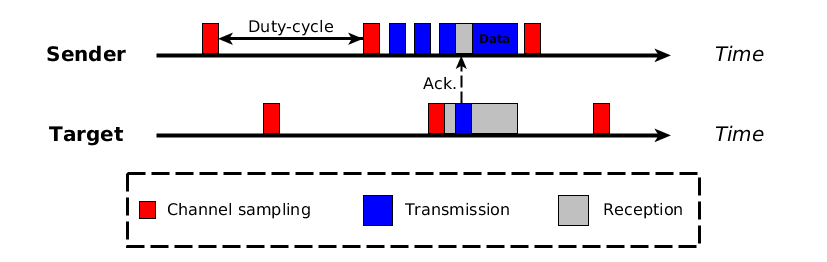
\includegraphics[width=0.8\textwidth]{figs/DC.png}
	\caption{Duty-cycling in preamble-sampling MAC protocols: the example of X-MAC.}
	\label{RW_dutycycle}
	\end{centering}
\end{figure*}

Communication performance and energy consumption are both directly correlated to the duty-cycle. Indeed, the shorter its value the higher the throughput, channel availability, energy usage, and the lower the average delay. In overall, energy savings performed through radio duty-cycling thus come at the cost of reduced performances, and vice-versa.

At the same time, the network has to evolve in a dynamic and unpredictible environment. Indeed, many  factors may vary over time and cause severe changes in the communication performance. To name a few, traffic patterns and load may vary due to sensing activity changes (e.g. event-driven and query-driven sensing approaches), and per-hop communication performances can be drastically affected by parameters such as temperature, air humidity and human activity \cite{linkstability12, addvalue13, tempimpact10}.
In this context, meeting both network lifetime and performance requirements at the same time is a very complex task, and smart mechanisms have to be designed to dynamically adapt the MAC configuration (i.e. the value of the duty-cycle) to changes in the network.% Indeed, both requirements are antinomic, and the ideal local MAC configuration of each node must

\subsection{Related work}

 %pTunes\cite{zfm12ptunes} for instance, information about the networks status (e.g. traffic load, loss-rate, delays) is added to data packets, using piggybacking. Over the successive packet receptions, the sink updates network statistics and computes a MAC configuration corresponding to the actual state of the network. Then, it broadcasts this value to the whole network, so that each node can fit to it. 

In order to solve this open problem, several approaches have been proposed. pTunes \cite{zfm12ptunes} for instance, dynamically adapts the MAC configuration throughout the network depending on the traffic load. Along with every message sent to the sink, information about the network state (e.g. traffic load, loss-rate, delays) is added, using piggybacking. Over the successive packet receptions, the sink updates network statistics and computes a single MAC configuration corresponding to the actual state of the network. Then, it broadcasts this value to the whole network. 
This approach provides gains in terms of performances (e.g. delays, loss-rate) as the network will dynamically adapt to any change of state. Yet, this scheme works in a centralized fashion to adapt the nodes MAC configuration globally, providing identical parameters simultaneously to each of these. Thus, the nodes being configured homogeneously over the network, pTunes could fail to precisely address local traffic load changes. pTunes also induce significant traffic overhead for performance monitoring and configuration broadcasting. 


Other solutions perform similarly, but provide each node with a specific MAC configuration. For instance, CLAC \cite{ecc12cross}, a Cross Layer Adaptation of Check intervals, uses packet flows to evaluate the delay of a multi-hop path, as well as per-link delay along this path. From this information is deduced a duty-cycle value. Such configuration is then propagated to each node along the path. Yet, as for pTunes, CLAC relies on a central decision made at the sink station, and the propagation of configurations at the scale of the whole network. This approach thus induces important control-trafic load, that may endanger network performance, and are hardly scalable.

%Other approaches rely on local decisions only to deduce the 

Paralelly, mechanisms have been developed to locally adapt the nodes configuration in reaction to network dynamics. In particular, \cite{mh10duty} presents AADCC, an Asymmetric Additive Duty Cycle Control algorithm.
%two algorithms for Duty-Cycle adaptation in WSN : Asymmetric Additive Duty Cycle Control (AADCC) and Dynamic Duty Cycle Control (DDCC).
AADCC takes inspiration from the 802.11 MAC protocol, replacing the multiplicative increase/linear decrease back-off by an asymetric linear increase/decrease scheme to avoid disruption in the network. Whenever five consecutive packets are successfully sent to the destination, the node increases its LPL by 100ms. Otherwise, each failed packet engender a 250ms LPL decrease. 
%On the other hand, DDCC uses several parameters (e.g. energy consumed) and their change vectors in a cost function to reach optimal LPL configuration.


%\cite{mh10duty} presents two algorithms for Duty-Cycle adaptation in WSN : Asymmetric Additive Duty Cycle Control (AADCC) and Dynamic Duty Cycle Control (DDCC). AADCC take inspiration from the 802.11 MAC protocol, replacing the multiplicative increase/linear decrease back-off by an asymetric linear increase/decrease scheme to avoid disruption in the network. Whenever five consecutive packets are successfully sent to the destination, the node increases its LPL by 100ms. Otherwise, each failed packet engender a 250ms LPL decrease. 
%On the other hand, DDCC uses several parameters (e.g. energy consumed) and their change vectors in a cost function to reach optimal LPL configuration.

%\cite{wwx10dynamic} presents DutyCon, a control theory-based dynamic duty cycle control approach. It decomposes the end-to-end delay guarantee problem into a set of single-hop delay guarantee problems along each data flow in the network.
%The authors suppose all data-flows to be disjoint (i.e. routing path from a source to the sink is not shared with other sources routing path). They extrapolate the end-to-end delay information from single-hop delay information. To do so they took into account the link delays as well as its PRR and Duty-Cycle period. Using a specific equation with these parameters, a new Duty-Cycle value is attributed to the node, in order to fit with the end-to-end delay requirement.

%DutyCon performances were evaluated both by simulation using NS-2 and by experimentation. The experimental testbed used in this article is composed of 7 Tmote Sky motes deployed in  a linear topology. One node is considered as being the sink, one as the source (which periodically sends packets), the remaining nodes being dedicated to forwarding packets only. The authors demonstrate that DutyCon is able to fit the networks end-to-end delay with the requirement, still reducing the average duty-cycle. However, the experimental setup is too specific to draw any general conclusion from these results.By simulation, the authors compared DutyCon with  two mechanisms extracted from the litterature, STS and DTS. DutyCon obtain otain results very close to STS in term of end-to-end delay, whatever the delay requirement, and is also more energy-consuming (except with very low delay requirement).
%DutyCon propose a dynamic duty cycle control approach, that aim at fitting with an end-to-end delay requirement provided by the user. However, DutyCon is based on several unrealistic assumptions (disjoint flow path), and do not provide any improvement compared to existing contributions.

\section{Core concept description}
\label{contrib}

In a context where parameters such as traffic load, communication performance and position in the routing structure may vary from one node to another and over time, finding the best-suited MAC configuration complying with the deployment needs at all time is a very complex task.
To cope with this phenomenon, we present CLIMAX, a framework that:

\begin{itemize}
	\item[1) ] defines achievable local constrainsts, derived from global requirements provided to the framework in the form of a set of key performance metrics of real-world applications: end-to-end delay, end-to-end-reliability and network lifetime;
	\item[2) ] passively monitors a range of performance metrics, that are directly impacted by the node MAC configuration or provide meaningful information on the network and node state;
	\item[3)] ~makes use of the above-mentionned information along with an evolutive model depicting the local communication behavior, to precisely calculate the best-suited MAC configuration among a pre-defined set and according to the current situation.
\end{itemize}

This way, CLIMAX dynamically calculates the MAC configuration of each node in the network, in a fully localized fashion and without any message overhead.

%To cope with this phenomenon, we present CLIMAX, a framework that passively monitors the network and find the best-suited MAC parameters accordingly, to fulfill global requirements dictated by the application. These requirements are provided to the framework in the form of a set of key performance metrics of real-world applications: end-to-end delay, end-to-end-reliability, power usage and network lifetime. Then, the CLIMAX framework passively collects relevant information about the network conditions and node status, that may impact one or several of those metrics. Finally, the framework relies on a multi-objective optimization problem (MOP) based on a radio communication model to calculate the best-suited MAC configuration.

\subsection{Global requirements definition}

Each WSN deployment has to fulfill certain requirements to be considered successful. Such requirements are specific to each application and are usually impossible to address altogether with an homogeneous and/or static network configuration.
In the present work, we consider a subset of generic applicative requirements, that are often encountered in typical WSN deployments: network lifetime, end-to-end delay and end-to-end resilience. However, any other specific requirement (e.g. data redundancy) can be provided to the framework.\\

\textbf{Network lifetime:} Many WSN have to operate autonomously for long periods. As they are often equipped with batteries and/or little-scale harvesting devices, their energy consumption has to be mitigated to fit with the global network lifetime requirement. We here refer to lifetime as the period during when no sensor is expected to fail due to battery depletion.

\begin{small}
\[
Life_{N} = \min_{n \in N} (Life_{n})
\]
\end{small}

with $Life_{N}$ the network lifetime and $Life_{n}$ the lifetime of a node $n$ in the network. Locally, this criterion thus corresponds to the time the considered node can last with its current energy consumption (or difference between energy usage and gains for energy harvesting nodes) considering its remaining energy reserves, or:

\begin{small}
\[
Life_{n} = NRJ / (T_{TX}(n) \times P_{TX} + T_{RX}(n) \times P_{RX} + T_{idle}(n) \times P_{idle})
\]
\end{small}

where $P_{TX}$, $P_{RX}$, and $P_{idle}$ are the current draws of the radio in transmit, receive, and idle mode, $T_{TX}(n)$, $T_{RX}(n)$, and $T_{idle}(n)$ are the fractions of time spent by a node $n$ in each mode, and $NRJ$ is the total amount of energy available. For specific deployments where the nodes can harvest some of their energy, the node lifetime corresponds to \\

\begin{small}
\[
Life_{n} = NRJ / (Usage(n) - Gain(n))
\]
\end{small}

where Gain(n) is the amount of energy harvested per time unit and Usage(n) is the amount of energy used per time unit with the current MAC configuration.\\

%, and power usage limit to the energy consumption threshold beyond which a node .

%\textbf{Power usage limit:} In some WSN deployments, node have an physical power usage limit, above which the electronic devices composing it may fail. In particular, very tiny sensor nodes, such as those used for animal monitoring for instance, have to cope with this limitation at all cost. In this context, no sensor node should exceed the power usage at any time during the deployment.

%\textbf{Delay tolerance:} Some applications have strong end-to-end delay constraints, so that reaction can be taken upon the detection of a specific event. For instance, patient-monitoring applications necessitate immediate notification of at-risk symptoms so that medical personnel can intervene in time.

%\textbf{Reliability tolerance:} Finally, in some deployments, collected data may be critical, and only a certain proportion of the data may be lost. For instance, most scientific applications require any meaningful event to be monitored, and thus require the loss-rate to be as low as possible.

\textbf{Quality of Service tolerance:} In some deployments, collected data may be critical. Its delivery must be both reliable and within stong time bounds, so that immediate reaction can be taken upon the successful detection of a specific event. For instance, patient-monitoring applications necessitate quick response to precise risk-assesment so that medical personnel can intervene in time. In practice, these requirements are portrayed by end-to-end delay and packet reception rate (PRR) constraints.\\
To be locally computed, these global QoS requirements (referred here as $Thresh$) need to be reduced to per-hop constraints. 
As the delay along a routing path (i.e. from the considered node to the sink, $Del_{e2e}$) is the sum of the delay of all per-hop link constituing it, the maximal delay of the outgoing link of a node $N$ hop away from the sink ($Dek_{N}$) can be deduced as follows:
\begin{small}
\[
Del_{e2e} \Leftrightarrow \sum_{x=1}^N D_{x} \Rightarrow \sum^N D_{N}
\]
\end{small}
and,
\begin{small}
\[
Del_{e2e} < Thresh \Rightarrow \sum^N D_{N} < Thresh \Rightarrow D_{N} < \frac{Thresh}{N}
\]
\end{small}
Thus, for a maximal delay defined as $Thresh$, a node $N$ hop away from the sink should ensure that the delay on its outgoing link do not exceed $\frac{Thresh}{N}$, by adapting its MAC configuration accordingly.
Similar calculations can be performed for the minimal PRR criterion ($PRR_{e2e}$): % is the product of the PRRs of all per-hop link constituing it, the minimal PRR of the outgoing link of a node $N$ hop away from the sink ($PRR_{N}$) can be deduced as follows:
\begin{small}
\[
PRR_{e2e} \Leftrightarrow \prod_{x=1}^N PRR_{x} \Rightarrow \prod^N PRR_{N}
\]
\end{small}
%supposing all links to be equals,
and,
\begin{small}
\[
   PRR_{e2e} > Thresh \Rightarrow \prod^N PRR_{N} > Thresh
\]
\[
 \Rightarrow PRR_{N} > \sqrt[N]{Thresh}
\]
\end{small}
%We define the end-to-end reliability $R$ as the average reliability of all paths P n .

%Some applications have strong end-to-end delay and reliability constraints, so that reaction can be taken upon the detection of a specific event

% end-to-end delay constraints, so that reaction can be taken upon the detection of a specific event. 

All the above-mentioned global constraints can be simply defined for the framework to use it. They can be either precise limitations (e.g. "$Network ~lifetime > 6 ~months$",  "$Loss ~rate < 80\%$") or loose ones (e.g. "$Maximize ~lifetime$",  "$Minimize ~delay$"), and are sorted by priority order.
%Each of those global constraint can be easily translated into local ones, so that each node can calculate its own MAC configuration without relying on any centralized decision.

% May consider soft constraints (range-like threshold) in addition to hard limitations? vague limits (maximize/minimize)?


%\subsection{Modeling framework}


\subsection{Network and node status monitoring}

In addition to applicative requirements, CLIMAX needs to be supplied with information about the current conditions the node evolves in. This information can be gathered through constant passive monitoring by each node of both the radio channel and node local state. 
In fact, each parameter that impacts at least one of the application-defined requirement has to be locally monitored by each node. We now provide some of the parameters that can be monitored and that have a direct impact on the requierements mentioned in the previous subsection.

\textbf{Position in the routing structure:} In typical data collection scenarios, a tree-shaped routing topology provides a unique path from every sensor node to a sink station. These paths are generally time-varying, as the routing protocol adapts them according to network dynamics. In this context, the distance in hops seperating a node from the sink station is a valuable information, that helps translating global communication performance requirements into per-hop constraints. Throughout the structure construction and adaptation, this information can be retrieved directly at the routing layer.

\textbf{Communication performance:} In addition to being a potential applicative requirement, the communication performance metrics (i.e. the PRR and delay) can also be monitored to estimate the current quality of a link and its evolution over time. %In addition, these metrics are highly dependant on the traffic load a node has to manage. The packet rate is thus also an important parameter to monitor.
%Together, these parameters help estimate the impact of MAC configuration changes and other monitored parameters on local performance, and thus better adapt it to fulfill global requirements.

%Communication performance are also highly dependant to the traffic load a node has to manage. The packet rate is thus also an important parameter to monitor and link with QoS 

%\textbf{Traffic rate:} Communication performance are highly dependant to the traffic load a node has to manage. as the MAC configuration dictates the packet rate able to be handled. This information 

%Each monitored parameter impacts performance othe concerned nodes 
%Climax thus performs a passive and constant monitoring of the following parameters.

%\textbf{Radio link quality:} The quality of a radio link can be reflected by a wide variety of parameters. In particular, most radio chipsets provide two physical-level indicators that could be used for this purpose: the Received Signal Strength Indication (RSSI, expressed in dBm) and the Link Quality Indicator (LQI). Although the RSSI value is identically calculated for all radio chipsets, LQI differs for each of them. The RSSI value is an estimate of the signal power level in the radio channel. For CC2420 radio chipsets, the LQI estimates how easily a received signal can be demodulated. Both these parameters are strongly correlated with communication performance (especially loss-rate, and to a lesser extent delay), as demonstrated in several prior studies.

\textbf{Energy usage:} Energy usage is often a critical parameter in WSN. Indeed, regulating energy consumption can help achieve lifetime goals as well as respect power usage boundaries. In order to do so, it is of prime importance to monitor the level and evolution of this energy consumption, as well as the amount of power remaining (i.e. the battery level). Several tools have been developed to provide precise monitoring of the energy usage \cite{dot07energest}, and are able to differenciate the source of energy consumption (e.g. Radio, CPU). % This information can  help predict the impact of MAC-layer configuration changes. %Each node then regulates its configuration so that its energy usage allow it sufficient autonomy to last more than dictated by the \textit{Network lifetime} requirement. %This information is crutial to comply with \textit{Network lifetime} requirement, as each node should adapt its energy usage to

\textbf{Traffic rate:} Both energy usage and communication performance are highly dependant to the traffic load a node has to manage. Indeed, an increased rate of messages sent to a node $N$ implies an increased channel occupancy that may lead to a local QoS reduction. Paralelly, sending messages induces extra energy usage that varies depending on the MAC configuration. This metric is thus of prime importance, and must be taken into account together with other metrics to derive the best-suited MAC configuration.

%\textbf{Packet transmission:} Packet transmission rate, avg preamble size

\subsection{MAC layer auto-adaptation}

\begin{figure*}[t]
	\begin{centering}
	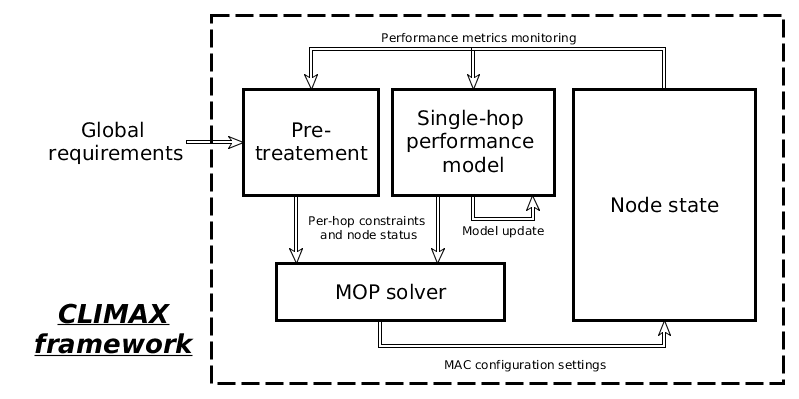
\includegraphics[width=0.8\textwidth]{figs/CLIMAX.png}
	\caption{The CLIMAX framework}
	\label{core_climax}
	\end{centering}
\end{figure*}

Before the deployment, the CLIMAX framework is provided with a set of MAC configurations, selected by the end user. Among this set, CLIMAX will will select the best-suited parameters to fulfill the node tasks. The framework also integrates an evolutive model, depicting the expected local performance (i.e. single-hop delay, single-hop PRR, node energy consumption) according to the traffic load and this set of considered MAC parameters.

During the network operation, the CLIMAX framework checks whether all of its per-hop constraints, previously derive from global requirements, are respected. Should this not be the case, the current performance and traffic load measured through the constant node monitoring are provided as parameters to to perfomance model. For each constraint, the model will then return the subset of duty-cycle values that are expected to fulfill it, sorted by order of performance. These lists are then provided to a solver, that will eventually select one of it as the node MAC configuration.

\subsubsection{Empirical per-link performance matrix}
\label{empir-matrix}
\textit{Default values can be derived from simulations/experiments led prior to the real deployment.}

\subsubsection{Markovian modeling}
\label{markov-matrix}
Another approach for calculating the default parameters of the evolutive model is to do so through Markovian modeling. Contrary to the empirical approach, a formally modeling expected per-link performance does not require any additional experimentation, and can thus be more convenient in many cases.

In order to theoretically calculate the per-link performance matrix, we rely on the same methodology as introduced in \cite{yang11}. For the sake of clarity, the channel is assumed to be free of fading, capture effect and hidden terminal. 

\subsubsection{Calculating the best-suited configuration}

To finally select a single best-suited MAC configuration, the solver considers each per-hop constraint iteratively, by priority order. Starting from the original list of all possible configurations, it removes at each step all the ones that do not fulfill the considered constraint. Then, when all constraints have been considered or when a single item remains in the list, the duty-cycle value that best complies with the first constraint (e.g. on top position of the first list) is chosen and provided to the current node for reconfiguration. Figure \ref{core_climax} illustrate the global functioning of the CLIMAX framework.% In addition, Equation \ref{core_equation} reviews in detail the MAC configuration selection process.

The performance model on which the CLIMAX framework relies to determine the new MAC configuration of a node is designed to evolve throughout the deployment, and improve over time to better correspond to the actual perfomance encountered by the node during the deployment. At first, it relies on default values obtained through analysis led prior to the WSN deployment (c.f. sub-sections \ref{empir-matrix} and \ref{markov-matrix}). Although inaccurate, these values allow CLIMAX to operate even during the first stages of the deployment, and adapt the nodes configuration for improved performance in this critical period, contrary to other approaches \cite{zfm12ptunes, ecc12cross, mh10duty}. In addition, the recorded performance metrics are also used to update the models, and better depict the actual communication behavior observed in reality. This way, over time, the model represents more and more accurately the condition the node  evolves in.

\section{Performance evaluation}
\label{results}

In this section, we present the performances of the CLIMAX framework. All the provided results were obtained via simulation campaigns carried out using the Cooja simulator \cite{?}.
The CLIMAX source code used in our evaluation campaign is available at \cite{?} for cross validation.
%\subsection{Evaluation setup}

\subsection{Expected local performance model}

In order to operate, the framework needs to be provided with a model, depicting the expected performance of a node single-hop communications. At first, the model relies on default values derived from evaluation campaigns conducted beforehand. These values allow the framework to function even during the first stages of the deployment. Over time, these inaccurate values are replaced by measures obtained throughout the deployment itself.

To provide our implementation of the CLIMAX framework with such default values, we performed an analysis of per-hop loss rate, per-hop delay and energy, depending on received traffic rate and MAC config.

\subsection{Framework validation}

%\subsection{Discussion}

\section{Conclusions and future work}
\label{ccl}

% Think about X-MAC results

\bibliographystyle{ieeetr}
\bibliography{autoconf}

%\begin{thebibliography}{0}
%
%\end{thebibliography}

%% biography section
%\begin{IEEEbiography}{Michael Shell}
%Biography text here.
%\end{IEEEbiography}
%
%% if you will not have a photo at all:
%\begin{IEEEbiographynophoto}{John Doe}
%Biography text here.
%\end{IEEEbiographynophoto}

% that's all folks
\end{document}
